\newpage
\section{Auswertung}


\subsection{Mittlere freie Weglänge}
\noindent
Als erstes wird für den Quecksilberdampf für die unterschiedlichen, für den Versuch genutzten Temperaturen, die mittlere freie Weglänge berechnet.\\
Dafür wird folgende Gleichung genutzt:

\begin{equation*}
    \bar{\omega}=\frac{0.0029}{5.5 \cdot 10^7 \symup{e}^{\frac{-6876}{T}}}
\end{equation*}

\noindent
Dabei sind hier die Temperaturen in Kelvin, der Druck in $\si{\milli\bar}$ und die Weglängein $\si{\centi\metre}$.\\
Die daraus errechnte mittlere frei Weglänge kann dann ins Verhältnis zur Entfernung zwischen Kathode und Beschleunigungselektrode gesetzt werden.
Diese entspricht hier $\SI{1}{\centi\metre}$. $\bar{\omega}$ sollte dabei im Idealfall um einen Faktor $1000$ größer sein.\\
Die Ergebnisse der Rechnungen sind in Tabelle \ref{tab:1} zu finden.

\begin{table}[h]
    \centering
    \small
    \begin{tabular}{S [table-format=3.2] S [table-format=1.9] S [table-format=5.2]}
        \toprule
        {$T \mathbin{\scalebox{1.5} / }\si{\kelvin}$} & {$\bar{\omega} \mathbin{\scalebox{1.5} / } \si{\centi\metre} $} & {$\frac{a}{\bar{\omega}}$}\\
        \midrule
        293.65 & 0.7786      &    1.28 \\
        421.15 & 0.000649593 & 1539.42    \\
        455.15 & 0.000191853  & 5212.32    \\
        \bottomrule
    \end{tabular}
\caption{Die Werte der mittleren freien Wegglänge mit der kdazu korrespondierenden Temperatur und im Verhältnis mit der Länge Beschleunigungsstrecke. }
\label{tab:1}
\end{table}


\subsection{Differentielle Energieverteilung}

\noindent
Nun werden die vom x-y-Schreiber erstellten, in Abbildung \ref{img:mess1} dargestellten, Messreihen untersucht.\\
Dafür wird aus aufgezeichneten Bremsspannungswerten für die Zeichnung gemittelt wie viel Volt ein Zentimeter entspricht.
Damit kann anschließend die Steigungen der Grafen in Abhängigkeit der Spannung untersucht werden.\\
Daraus können Rückschlüsse über die Menge und Energie der regristrierten Elektronen geschlossen werden.\\\\
Zu erst ergibts sich also gemittelt ein Wert von $\SI{0.40(4)}{\volt\per\centi\metre}$ in den Messwerten.\\
Mit Hilfe von Steigungsdreiecken lässt sich daraus dann für die jeweiligen Spannungen die korrespondierende Steigung ablesen.\\
Für die Messungen bei $T_1=\SI{20.5}{\celsius}$ mit der Bremsspannung $U_1$ und $T_2=\SI{148}{\celsius}$ mit $U_2$, sind die Ergebnisse in Tabelle \ref{tab:2} dargestellt.\\
Grafisch findet sich das ganze in den Abbildungen \ref{img:1} und \ref{img:2} wieder.


\begin{table}[h]
    \centering
    \small
    \begin{tabular}{S [table-format=1.3] S [table-format=1.2] S [table-format=1.3] S [table-format=1.2]}
        \toprule
        {$U_1 \mathbin{\scalebox{1.5} / }\si{\volt}$} & {${\frac{\increment y}{\increment x}}_1  $} &{$U_2 \mathbin{\scalebox{1.5} / }\si{\volt}$}& {${\frac{\increment y}{\increment x}}_2  $}\\
        \midrule
        0        & 0.2  & 0        & 1.2  \\
        0.199 & 0.15 & 0.199 & 1.45 \\
        0.599 & 0.2  & 0.599 & 1.35 \\
        0.999 & 0.25 & 0.999 & 1.35 \\
        1.399 & 0.2  & 1.399 & 1.3  \\
        1.799 & 0.2  & 1.799 & 1.15 \\
        2.199 & 0.3  & 2.199 & 1.05 \\
        2.599 & 0.3  & 2.599 & 0.75 \\
        2.998 & 0.4  & 2.998 & 0.25 \\
        3.398 & 0.4  & 3.398 & 0.2  \\
        3.798 & 0.65 & 3.798 & 0.2  \\
        4.198 & 0.7  & 4.198 & 0    \\
        4.598 & 0.65 & 4.598 & 0    \\
        4.998 & 0.85 & 4.998 & 0    \\
        5.397 & 1.1  & 5.397 & 0    \\
        5.797 & 1.5  & 5.797 & 0.05 \\
        6.197 & 1.8  & 6.197 & 0.05 \\
        6.597 & 2.7  & 6.597 & 0    \\
        7.197 & 1.6  & 7.197 & 0    \\
        7.597 & 0.7  & 7.597 & 0    \\
        8.196 & 0.5  & 8.196 & 0.05 \\
        8.196 & 0.05 & 8.196 & 0.05 \\
        \bottomrule
    \end{tabular}
\caption{Die Werte der mittleren freien Wegglänge mit der dazu korrespondierenden Temperatur und im Verhältnis mit der Länge Beschleunigungsstrecke. }
\label{tab:1}
\end{table}



\begin{figure}[H]
    \centering
    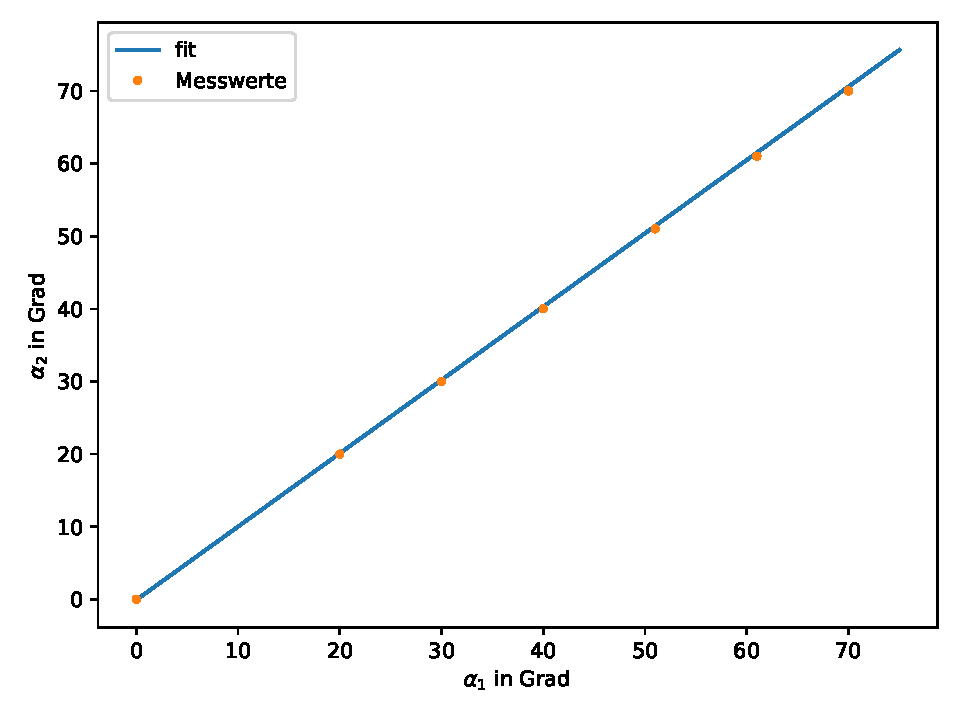
\includegraphics[width=0.6\textwidth]{build/plots/plot1.pdf}
    \caption{Die Steigung der differentiellen Energieverteilung in Abhängigkeit der Beschleunigungspannung bei $\SI{20.5}{\celsius}$.}
    \label{img:1}
\end{figure}

\begin{figure}[H]
    \centering
    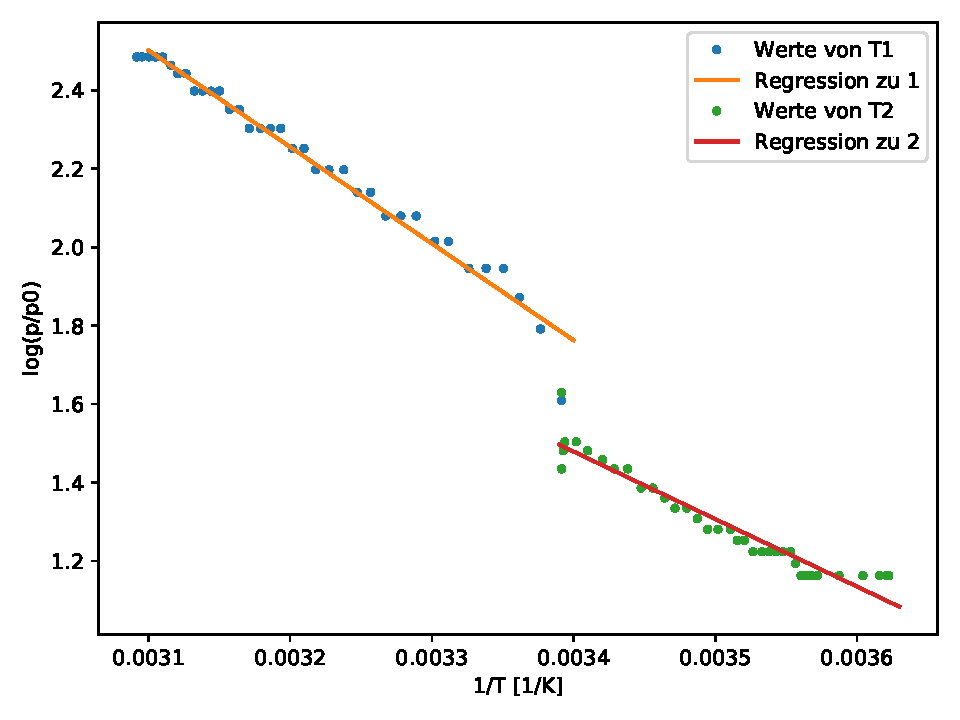
\includegraphics[width=0.6\textwidth]{build/plots/plot2.pdf}
    \caption{Die Steigung der differentiellen Energieverteilung in Abhängigkeit der Beschleunigungspannung bei $\SI{148}{\celsius}$.}
    \label{img:2}
\end{figure}

\noindent
Aus Abbildung \ref{img:1} lässt sich ablesen das fast alle Elektronen die Energie $\SI{6.6}{\eV}$ besitzen. 
Wenn dieser Wert vom der Beschleunigungsspannung von $\SI{12}{\volt}$ subtrahiert wird, ergibt sich das Kontaktpotential $k=\SI{5.4}{\volt}$.\\
Für die Messreihe mit der Gastemperatur $T_2=\SI{148}{\celsius}$ fallen die Steigungen sehr früh ab. 
Dies resultiert aus dem überschreiten der Anregungsenergie $E=\SI{4.9}{\eV}$\cite{theo}, wodurch Stoßprozesse stattfinde, die das Quecksilber bei gleichzeitigem Energieverlust der Elektronen, anregen.\\
Abzüglich des Kontaktpotentials ergibt sich in der Theorie ein Abfall des Graphen bei $\SI{-0.5}{\eV}$, was vor dem Beginn der Zeichnung wäre.


\subsection{Franck-Hertz-Kurve}

\noindent Auch für diese Messreihe wird erst wieder die Spannung pro Zentimeter gemittelt, was sich zu $\SI{2.10(8)}{\volt\per\centi\metre}$ ergibt.\\
Hier wird nun der Abstand zwischen den Peaks der Franck-Hertz-Kurve gemessen, daraus der Spannungsabstand bestimmt und damit dann die Anregungsenergie von Quecksilber errechnet.\\
Der Abstand der Maxima findet sich in Tabelle \ref{tab:3}. Gemittelt ergeben diese Werte einen Energieabstand der Maxima von $\SI{5.45(40)}{\eV}$.

\begin{table}[h]
    \centering
    \small
    \begin{tabular}{S [table-format=1.0] S [table-format=1.1] S [table-format=1.5]}
        \toprule
        {Grad der Maxima} & {$\text{Abstand} \mathbin{\scalebox{1.5} / } \si{\centi\metre} $} & {$\text{Energiedifferenz } \mathbin{\scalebox{1.5} / } \si{\eV}$}\\
        \midrule
        1 & 2.4 & 5.03319 \\
        2 & 2.4 & 5.03319 \\
        3 & 2.6 & 5.45262 \\
        4 & 2.5 & 5.2429  \\
        5 & 2.7 & 5.66233 \\
        6 & 2.6 & 5.45262 \\
        7 & 3   & 6.29148 \\
        \bottomrule
    \end{tabular}
\caption{Die Abstände der Maxima der Franck-Hertz-Kurve zu nächsten und die daraus resultierende Energiedifferenz zwischn den Maxima.  }
\label{tab:3}
\end{table}

\noindent Aus der gemittelten Energiedifferenz lässt sich über 
\begin{equation*}
    \lambda= \frac{\symup{c}\symup{h}}{\increment E}
\end{equation*}
berechnen. Dabei ist $\symup{c}$ die Lichtgeschwindigkeit\cite{c} und $\symup{}$ das Planck''sche Wirkungsquantum\cite{Planck}.\\
Damit ergibt sich $\lambda=\SI{227.385}{\nano\metre}$.\\
Der Energieverlust von Elektronen beim zentralen elastischen Stoß ist hier zu vernachlässigen, da die Elektronen bei nicht zentralen Stößen praktisch keine Energie verlieren.\\
Es entsteht dort nur eine Richtungsänderung und da es hier nur um den Ort der Maxima geht und nicht um ihre Höhe sind diese Vorgänge zu vernachlässigen.
